\documentclass{standalone}
\usepackage{tikz}
\usepackage{ctex,siunitx}
\setCJKmainfont{Noto Serif CJK SC}
\usepackage{tkz-euclide}
\usepackage{amsmath}
\usetikzlibrary{patterns, calc,3d}
\usetikzlibrary{decorations.pathmorphing,decorations.pathreplacing,decorations.shapes}
\begin{document}
\small
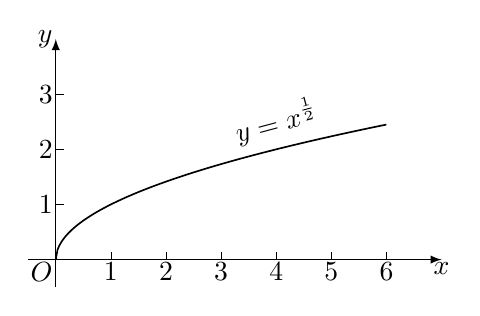
\begin{tikzpicture}[>=latex,scale=0.7,inner sep=1pt]
  \draw[->](-0.5,0)--(7,0)node[below]{$x$};
  \draw[->](0,-0.5)--(0,4)node[left]{$y$};
  \node at (0,0)[below left]{$O$};
  \foreach \x in {1,...,6}
  {
    \draw[very thin](\x,0)node[below]{$\x$}--++(0,0.14);
  }
  \foreach \x in {1,2,3}
  {
    \draw[very thin](0,\x)node[left]{$\x$}--++(0.14,0);
  }
  \draw[semithick,samples=200,domain=0:6.0]plot(\x,{sqrt(\x)});
  \node at (4,2.5)[rotate=15]{$y=x^{\frac12}$};
\end{tikzpicture}
\end{document}